\chapter{Automation}\label{chapter:Automation}
In the last chapter, we considered a representation for incidence claims involving lines and planes which helped us write shorter verifications. The use of these rules also appeared ripe for automation. 

The HOL~Light theorem prover expects its users to work ``close to the metal'', often writing ML directly. Writing new tools can be comfortable in this environment, and it is easy to prototype and experimentally integrate new tools into the rest of the system and existing proof languages. In this chapter, we shall see how this integration can take the form of a concurrent and collaborative automated tool for incidence reasoning, which can be made available as a tactic and in Mizar~light proof steps.

Much of this chapter and the subsequent chapter is an expansion and improvement on earlier work~\cite{ScottExploring,ScottComposable}.

\section{Related Work}
As far as fully automated theorem proving goes, the oldest successes are probably in geometry. The signed-area method \cite{MachineProofsInGeometry} of Chou et al, proved to be particularly capable at finding large numbers of non-trivial geometric theorems. But in this section, we restrict our attention to automation that can apply to the very basic incidence theory we consider here. The signed-area method, which typically assumes an ordered field, is already outside of our scope.

\subsection{Wu's Method}
When considering general automation in Hilbert's \emph{Foundations of Geometry}, there is probably no work more relevant than Wu's method~\cite{WuMechanicalTheoremProving}. Wu credited the \emph{Foundations of Geometry} for the metatheoretical insights that led to his mechanisation procedure for the whole of geometry\footnote{Wu was possibly giving Hilbert too much credit}.

One of Wu's own insights was that the method of proof in a synthetic geometry system such as Hilbert's often falls short of absolute rigour because degenerate cases are routinely missed. Typically, when we state axioms and theorems for some geometric figure, we have in mind a particular ``genericity'' of that figure which is hard to capture formally. Moreover, the axioms and theorems may admit some generalisation to what we would regard as ``degenerate'' cases, even if this is not immediately clear at the time. We have already seen in the last group that some of Hilbert's axioms, such as Axiom~\ref{eq:g11} hold in degenerate cases (though this does not imply that the axiom should be made \emph{stronger}). We shall show in Chapter~\ref{chapter:HalfPlanes} how the particularly troublesome Axiom~\ref{eq:g24} (troubling at least as far as incidence reasoning is concerned) can be strengthened by allowing degenerate cases.

But ``degenerate'' is not well-defined, and it is not always clear how the conditions of a theorem can be relaxed. Moreover, when trying to rule out certain degenerate cases, there are plenty that are easily missed. When we formalise, we cannot simply neglect them unless we have proof tools that can do it for us. Filling in all the gaps requires enormous effort and complication of the proof, so it would seem that Wu is correct: we cannot be truly rigorous unless we can systematically deal with degenerate conditions. This provides an alternative way to diagnose the gaps in Hilbert's proofs spotted by Meikle and Fleuriot~~\cite{MeikleFleuriotFormalizingHilbert}: they were gaps concerning degeneracy conditions about point incidence.

Wu's highly celebrated method automatically inserts non-degeneracy conditions to the theorems it proves, and if possible, it automatically deletes redundant conditions to make a specific theorem more generic. The method has been used to automatically prove an enormous number of non-trivial theorems in unordered geometry \cite{MechanicalGeometryTheoremProving}. To cover ordered geometry, Wu appealed to the embedding of Euclidean geometry in real-closed fields, for which Tarksi has a well-known decision procedure. The method has much less success here, owing to the gross intractability of the decision procedure~\cite{TarksiMcNaugtonReview}. 

Unfortunately, Wu's automation is not particularly appropriate for our own work. If we were to exploit it, we would need to show how each of his mechanical steps can be reduced to the axioms of Hilbert's system. But this reduction will presuppose some of the very elementary theorems which we are trying to mechanise. Indeed, Wu's method is based at least on results which rest on Desargues' theorem --- Theorem~53 in the \emph{Foundations of Geometry}. Furthermore, our focus in the present work is \emph{ordered geometry}, a domain in which Wu's method is ill-suited. 

\subsection{Ranks}
For the specific problem of incidence reasoning, Magaud et al's work~\cite{RankDesargues} is closest in spirit to our own. It too, is based on point-sets, but the authors have beautifully abstracted the core idea. 

Several of our rules for lines and planes in Figure~\ref{fig:PointSets} in the last chapter appear analogous. Magaud et al have captured the analogy formally using \emph{ranks}. The rough idea is that an $n$-dimensional set is assigned a rank of $n+1$. There are then key rules which assert that, given point sets $X$ and $Y$, the sum of the ranks of $X \cup Y$ and $X \cap Y$ is no greater than the sum of the ranks of $X$ and $Y$. This abstractly characterises our rule for taking the union of collinear and planar sets. 

Magaud's approach allows the author's to generalise to arbitrary dimension, and the elegance of the theory helps us see our own approach as less ad-hoc than it might otherwise. For the rest of this chapter, however, we shall focus on our original, more concrete representation.

\section{Inference Rules}
The rules from Figure~\ref{fig:PointSets} tell us how to reason with finite collinear and planar sets, and so can form the basis of a combinatorial algorithm. Our rules trade in four kinds of theorem: theorems about which points are distinct, which points are collinear, which triples are non-collinear, and which points are planar. These theorems will be the domain of our algorithm, whose chief procedures will be based on rules to interderive them.

Our rules already show how to introduce collinear and planar sets. Additionally, we need ways to derive the inequalities and triangles on which the rules depend. Firstly, we note that any triangle or non-collinear triple implies the mutual distinctness of its three points, giving us one way to introduce point inequalities. Another way to derive inequalities is through simple congruence reasoning: suppose we have a collinear set $S$, and a non-collinear triple sharing two points with $S$. Then the third point of the triple must be distinct from all points in $S$. 

Next, we need to introduce non-collinear triples. We based our method here on patterns of reasoning that showed up in our Isabelle formalisation. Suppose we have a collinear set $S$ and a non-collinear triple sharing two points with $S$. Then the third point forms a non-collinear triple with all pairs of points in $S$ known to be distinct.

Finally, we consider how we might infer when two points are \emph{equal} using our rules. Again, we followed a pattern of argument that showed up in the Isabelle formalisation. Given two collinear sets $S$ and $T$, which have a non-collinear union, we can infer that their intersection must be empty or a singleton. So if the intersection is a set of points $\{P_1,P_2,\ldots,P_n\}$, then we know immediately that these points are identical. This, we noted in the last chapter, is just telling us that distinct lines intersect in at most one point, as per Hilbert's Theorem~1.

We now summarise the rules and methods for introducing new theorems. 
\begin{itemize}\label{list:Procedures}
\item[$\code{ncolneq}$] Infer inequalities from non-collinear triples:
\begin{displaymath}
\neg\code{collinear}\ \{A,B,C\} \implies A \neq B \wedge A \neq C \wedge B \neq C.
\end{displaymath} (by rule \ref{rule:colltwo});
\item[$\code{colncolneq}$] Infer inequalities from a collinear set containing two points of a non-collinear triple. 
\begin{align*}
  &\code{collinear}\ S \wedge \neg\code{collinear}\ \{A,B,C\}\\
  &\qquad\wedge A,B\in S \implies \forall S. S \in As \implies C \neq S
\end{align*}(by rule~\ref{rule:collsubset}). For example, 
\begin{align*}
\code{collinear} \{A, B, C, D, E\} \wedge & \neg\code{collinear} \{A, B, P\}\\
&\implies C \neq P \wedge D \neq P \wedge E \neq P.
\end{align*}
\item[$\code{coleq}$]
Equate points in the intersection of two collinear sets which are jointly non-collinear.
\begin{align*}
&\code{collinear}\ S \wedge \code{collinear}\ T \wedge \neg\code{collinear}\ U \wedge U \subseteq S \cup T \\
&\qquad\qquad\wedge A,B \in S,T \implies A = B
\end{align*} (by rules~\ref{rule:collsubset} and \ref{rule:collunion}).
For example,
\begin{align*}\
&\code{collinear} \{A, B, C, D, E\} \,\wedge\,\code{collinear} \{A, C, E, X, Y\}\\ 
&\qquad\, \wedge\,\neg\code{collinear} \{A, B, Y\}\implies A = C \wedge A = E \wedge C = E.
\end{align*}
\item[$\code{colncolncol}$] Infer new non-collinear triples from a collinear set and another non-collinear triple.
\begin{align*}
  &\code{collinear}\ S \wedge \neg\code{collinear}\ \{A,B,C\}\\
  &\qquad\wedge X,Y,A,B \in As \wedge A \neq B\implies \neg\code{collinear}\ \{C,X,Y\}.
\end{align*} (by rules~\ref{rule:collsubset} and~\ref{rule:collunion}). For example,
\begin{align*}
A \neq C \wedge D \neq E &\wedge \code{collinear} \{A, B, C, D, E\} \wedge \neg\code{collinear} \{A, B, P\}\\
&\implies \neg\code{collinear} \{A, C, P\} \wedge \neg\code{collinear} \{D, E, P\}.
\end{align*}
\item[$\code{colcol}$] Use rule \ref{rule:collunion} to show that the union of collinear sets which intersect at more than one point is collinear.
\item[$\code{planeplane}$] Use rule \ref{rule:planeunion} to show that the union of planar sets intersecting at a non-collinear triple is planar.
\item[$\code{colplane}$] Use rule \ref{rule:collplane} to show that a collinear set is planar.
\item[$\code{colplaneplane}$] Use rule \ref{rule:collplaneplane} to show that the union of a collinear and planar set intersecting in at least two points is planar.
\item[$\code{colcolplane}$] Use rule \ref{rule:collcollplane} to show that the union of intersecting collinear sets is planar.
\end{itemize}

%We have stated these rules at the object level, and they can be applied exhaustively by just using matching and term-rewriting. However, we have also implemented them directly as ML inference rules. This is preferred for efficiency, since we can be smarter about when a match should fail, and we can alleviate the burden on the rewriter.

%With hard-coded ML inference rules, we can dispense with sets and represent our theorems as ordinary first-order terms. So $\code{collinear}\ \{A,B,C,D,E\}$ gets expressed directly as the existential produced by unfolding the definition of $\code{collinear}$ and the finite set constructors:
%\begin{displaymath}
%  \exists a. \code{on\_line}\ A\ a\wedge\code{on\_line}\ B\ a\wedge\code{on\_line}\ C\ a\wedge\code{on\_line}\ D\ a\wedge\code{on\_line}\ E\ a.
%\end{displaymath}
%The collinear union rule is now ML code which strips the existential and conjuncts from these formulas, and then directly applies existential rules and Axiom~\ref{eq:g12} to produce a new claim of collinearity of the same form. Our object level rules can serve as a weak sort of verification: after unfolding the predicates $\code{collinear}$ and $\code{planar}$ and unfolding the finite sets, direct matching should behave identically to our hard-coded ML.

%Besides efficiency, the fact that we stick to first-order means that our declarative proofs are not loaded down having to unfold statements involving $\code{collinear}$ and $\code{planar}$ predicates, nor do they have to perform any set-theoretic reasoning.

\section{N\"{a}ive Implementation}\label{sec:NaiveImplementation}
Our first prototype used basic forward-chaining, and such methods have been used with some success to investigate Hilbert's geometry~\cite{ForwardChainHilbert}. Forward chaining seemed particularly suitable for our use case. We have already noted that some of our proofs were suboptimal, that we believed Hilbert might have made errors in assuming certain non-degeneracy conditions, and so we wanted a tool which could \emph{explore} the proof space of incidence reasoning surrounding each of Hilbert's proofs. 
\
The idea of using forward-chaining in this sort of exploratory way also opened up the possibility of designing an automated tool which could \emph{collaborate} with the user as they develop a proof. Forward-chaining seemed quite apt, since its focus on continually growing a base of facts corresponds well with how a declarative proof is developed by continually growing a proof context. 

Our first algorithm worked on \emph{generations} made up of five lists, one for each of the different kinds of fact: point equalities, point inequalities, collinear sets, non-collinear sets, and finally planar sets. The procedures of \S\ref{list:Procedures} were then applied across all relevant combinations of theorems from the five lists, to produce a new generation of lists. In this way, the algorithm produces a sequence of generations, each a superset of its predecessor.

\subsection{Concurrency}\label{sec:NaiveConcurrency}
Typically, the automation available in interactive theorem provers is invoked on demand by the user when they evaluate individual proof steps. But when the user writes the formal proof for the first time, or comes to edit it later, they will spend most of their time \emph{thinking}, consulting texts, backtracking and typing in individual proof commands. The CPU is mostly idling during this process, and we can exploit this idle time to run automated tools concurrently.

The Isabelle Theorem prover has capitalised on this with Sledgehammer~\cite{IsabelleSledgehammer}. By invoking this command, the user can continue to work on a proof, while generic first-order tools are fired off as separate background processes, attempting to solve or refute the user's goals independently. If the tools reach a conclusion, the generated proof certificates can be automatically and seamlessly integrated into the user's proof-script. 

We argue that we can do one better, since it is almost trivial to turn our algorithm into something of a ``collaborative'' architecture. We are focusing on forward-chaining and declarative proof, and as we remarked, the way that a user builds a declarative proof is by growing a proof context towards a goal, while a forward-chaining algorithm interatively grows a set of facts. These processes are analogous, so why not splice the two? A user's proof script is then a user guided, manually crafted search through the proof space, but now one which has access to the derivations of a forward chaining algorithm. At the same time, the forward chaining algorithm works independently, but can freely incorporate the user's manually obtained deductions into its own base of facts. The two systems, the automation and the human user, can thus be seen as collaborating, sharing data as they both strive towards the goal. 

We started with a very simple implementation of this setup. We spawn a thread that is initialised with an empty generation of facts. New generations are produced iteratively through forward-chaining. At the same time, the thread  monitors the proof context, so that each time the user adds a hypothesis by performing a declarative proof step, the hypothesis can be automatically inserted into the current generation and used for further chaining.

The thread then echoes each generation of facts concurrently to a separate terminal, while the user works on the proof script. We then introduce a variable $\code{the\_facts}$ which is updated so that it always dereferences to the current generation. This variable can be used in a proof script to justify the current step with the automatically inferred facts. 

%When a fixpoint is detected, the user is notified, so that they can decide whether perhaps an assumption is missing, or whether a more sophisticated subproof is needed. In the meantime, the forward-chaining thread will sleep.

%Since we are using an LCF style prover~\cite{LCF}, we always ensure that our forward-chaining derivations are fully-expansive~\cite{FullyExpansive}. This means that to carry out its derivations, the tool directly applies inference rules to generate fully machine verified lemmas. These lemmas can then be seamlessly integrated into the user's proof script to produce a fully machine-checked proof.

\subsection{Discovery}
In our designs, our automation is very much intended in the spirit of \emph{assistance}. It is not intended to take over, or to solve the user's problems. It is there as a support, to be relied on as desired. These make its purposes so modest that it is not clear why such a tool would ever be needed. Perhaps it would be useful to set the scene.

We would typically develop our geometric proofs on paper, but as we noted above, a typical geometric diagram probably includes many non-degeneracy assumptions. In our case, these assumptions required that certain points be non-equal and others non-collinear. Discharging these assumptions typically meant a pen-and-paper combinatorial search, which we would again trace out on paper.

In this narrow domain, it was easy to imagine simple programs which could do the combinatorial search for us, and which could display a breadth of theorems in case we had missed shorter paths, or overlaps with later inferences. This, then, is not quite automated search, but more assisted search. We have chosen to give it the shorter title of ``discovery'', which stresses the point that we are usually interested in obtaining many results from the search process, including results we had not expected, and that we generally did not run the searches with a particular goal theorem in mind. However, we should mention that our use of the word ``discovery'' is to be contrasted with fully automated discovery systems which search for arbitrary interesting theorems and concepts without the need for assistance~(see the work of Colton et al~\cite{ColtonInterestingness}, as well as McCasland and Bundy~\cite{Mathsaid}).

\section{An Implementation in Combinators}\label{sec:DiscoveryAlgebra}
\subsection{Data-Flow}
Our prototype implementation was an adequate proof of concept, and enabled us to write some very short and clear proofs. We have some examples of these in the next chapter. However, our prototype currently has no theoretical underpinning. The finer details of the implementation are complex, ad-hoc, unlikely to scale, and cannot be easily modified to work on new problems. 

Much of the complexity of the ML algorithm comes from the fact that each generation of theorems is partitioned into five types: point equalities, point inequalities, collinear sets, non-collinear sets and planar sets. By partitioning in this way, we greatly reduce the number of combinations of theorems we need to try with each inference rule, but there is still much wasted effort. Every time a new generation is generated, all relevant combinations are applied, \emph{including} the combinations which were applied for the \emph{last} generation. Our simple lists do not help us filter out the repetitious work.

Rather than seeing the problem as simply one of repeating inferences across a succession of generations, we decided to model the data-flow directly. The flow of data for our problem, according to the rules of \S\ref{list:Procedures}, is given in Figure~\ref{fig:DataFlow}.

\begin{figure}
\centering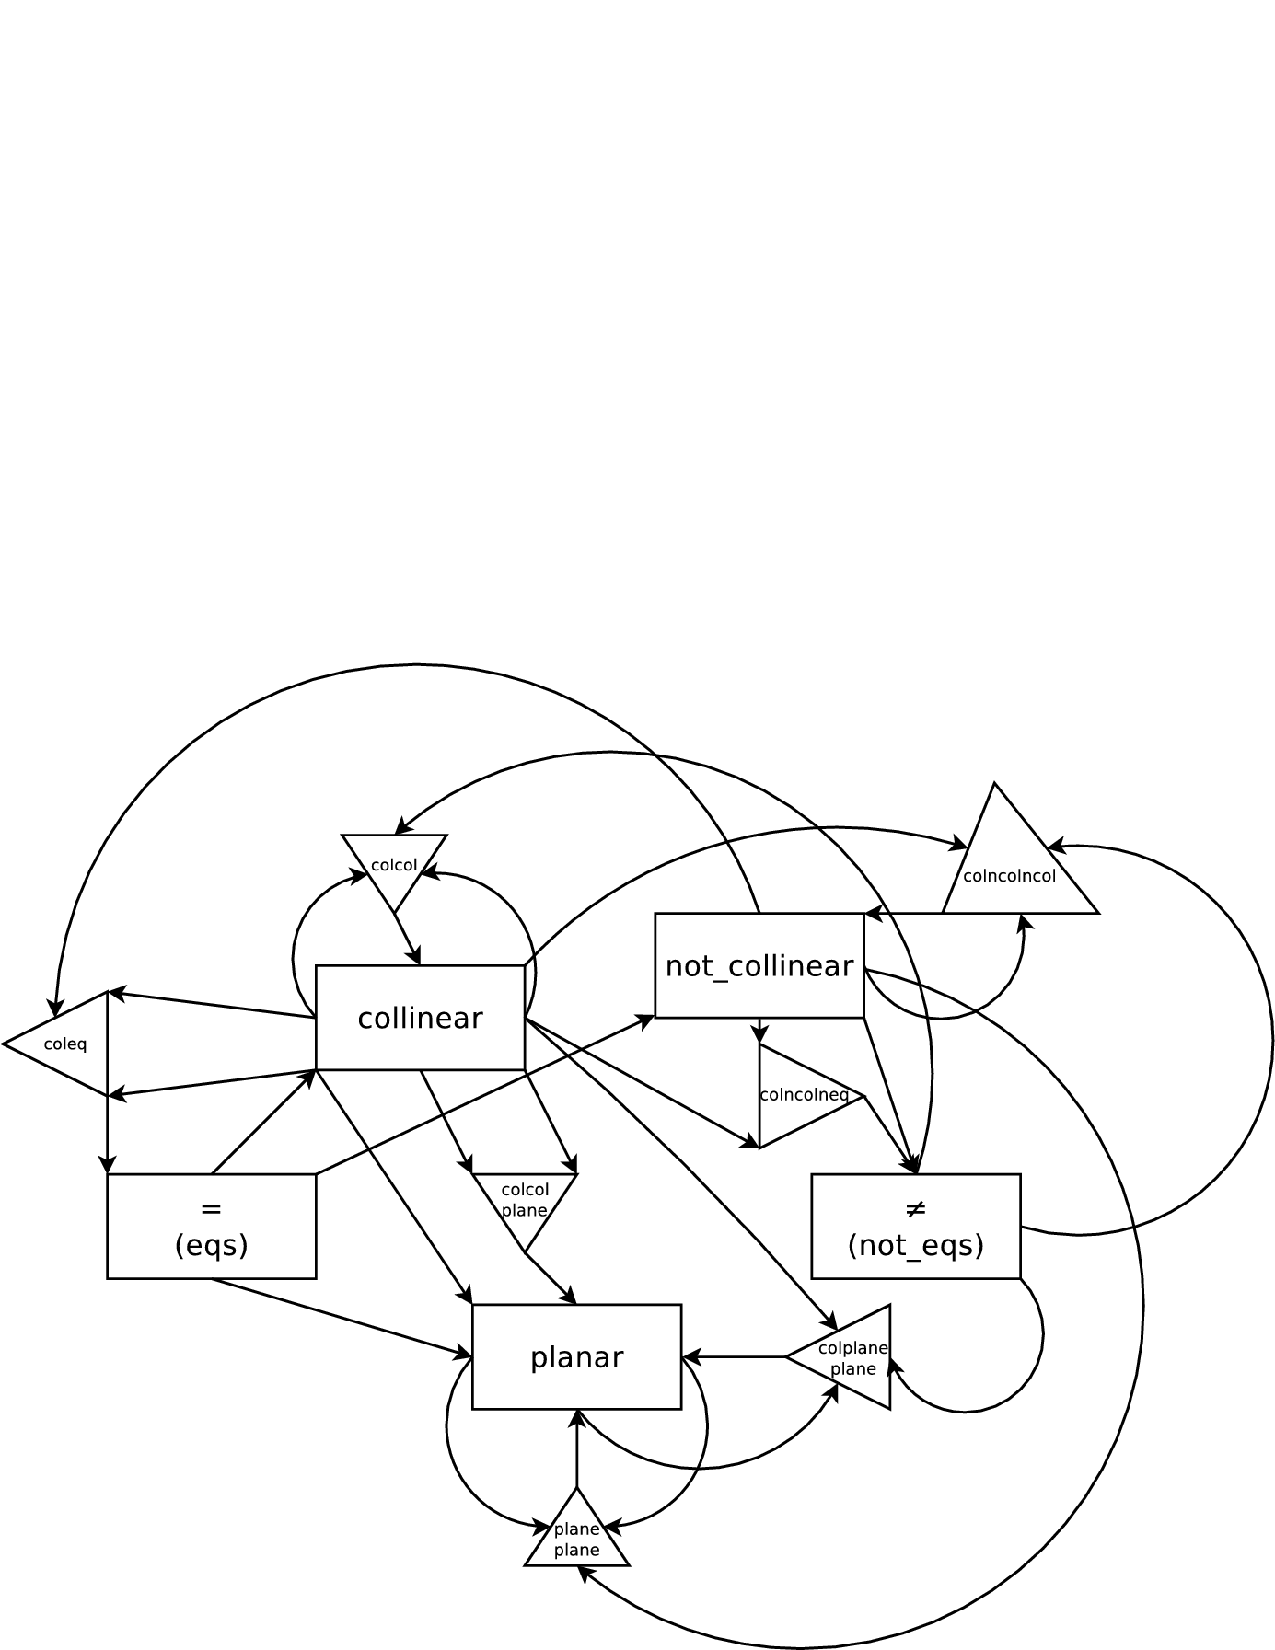
\includegraphics[scale=0.5]{automation/DataFlow}
\caption{Data-flow for incidence reasoning: boxes represent our collections of various kinds of theorem, while triangles represent inference rules}
\label{fig:DataFlow}
\end{figure}

The particular automation we need for Hilbert lies in a very narrow domain, and we would rather see it as a  ``one-shot'' tool, one which is unlikely to be needed in other projects. This makes it most similar in purpose to a hand-crafted conversion or tactic~\cite{Tactics}. Conversions and tactics, a staple of the LCF approach to theorem proving, are normally written and understood as combinators~\cite{CombinatorLanguages}, which are themselves a staple of strongly-typed functional programming. 

Our aim in this section will be to show how a data-flow such as that of Figure~\ref{fig:DataFlow} can be directly expressed in a suitable combinator language, with a distinguished set of primitives which can be combined by transformations. While the incidence automation itself will be a one-shot tool written in this language, we hope the data-flow language will be more useful in other contexts.

The advantage of choosing a combinator language, as opposed to some other kind of domain-specific language, is that it fully integrates with the host programming language, and is therefore easy to integrate with the tactic combinator language and the Mizar~Light combinator language. The user is also free to extend the language and can easily inject computations into it using lambda abstraction.

\subsection{Related Work}
The idea of an algebraic data-flow language was considered early on by Chen~\cite{ChenForwardChaining}, who gave a specification for a variety of primitives very similar to our own, though without an implementation. Since then, algebras for logic programming, handling unbounded and fair search have been developed~\cite{BacktrackingMonad}. The algebra we shall consider here is related and was originally conceived by Spivey~\cite{SearchAlgebras}. It has more rigorously developed underpinnings, and compared to other search algebras such as those of the logic programming monad~\cite{BacktrackingMonad}, it places stronger constraints on the order in which the values are generated. We shall be generalising Spivey's ideas somewhat, and also hope to give a more ``operational'' motivation for the definitions.

\subsection{Streams}\label{sec:Streams}
Our overarching purpose is to output a stream of theorems, perhaps to a terminal, to a database of facts to be used during a proof, or perhaps to another consumer for further processing. If we think of this output \emph{as} the implementation, then we are dealing with procedures which lazily generate successive elements of a list. These lazy lists, or streams, shall be the primitives of our data-flow algebra. 

For now, we leave unspecified what computations are used to generate the primitive streams. It might be that a stream simply echos a list of precomputed theorems; it might generate theorems using input data; it might generate them from some other automated tool. We shall focus instead on transformations for streams, and in how we might lift typical symbolic manipulation used in theorem proving to the level of streams.

One reason why lists and streams are a good choice is that they are \emph{the} ubiquitous data-structure of ML and its dialects, and have rich interfaces to manipulate them. A second reason why lists are an obvious choice is that they have long been known to satisfy a simple set of algebraic identities and thus to constitute a monad~\cite{MonadWadler}. We can interpret this monad as decorating computations with non-deterministic choice and backtracking search. 

Monads themselves have become a popular and well-understood abstraction in functional programming. Formally, a monad is a type-constructor $M$ together with three operations 
\begin{align*}
&\code{return} : \alpha \rightarrow M\;\alpha\\
&\code{fmap} : (\alpha \rightarrow \beta) \rightarrow M\;\alpha \rightarrow M\;\beta\\
&\code{join} : M\;(M\;\alpha) \rightarrow M\;\alpha
\end{align*}
satisfying the algebraic laws given in Figure~\ref{fig:MonadLaws}.

\begin{figure}
\begin{align}
&\code{fmap}\;(\lambda x.\;x)\;m = m\notag\\
&\code{fmap}\;f \circ \code{fmap}\;g = \code{fmap}\;(f \circ g)\notag\\
&\code{fmap}\;f \circ \code{return} = \code{return}\circ f\notag\\
&\code{fmap}\;f \circ \code{join} = \code{join} \circ \code{fmap}\;(\code{fmap}\;f)\notag\\
&(\code{join} \circ \code{return})\;m = m\notag\\
&(\code{join} \circ \code{fmap}\;\code{return})\;m = m\notag\\
&\code{join} \circ \code{join} = \code{join} \circ \code{fmap}\;\code{join} \label{eq:JoinAssoc}
\end{align}
\caption{The Monad Laws}
\label{fig:MonadLaws}
\end{figure}

The list monad can be used for search, but takes list concatenation $\code{concat} : [[\alpha]] \rightarrow [\alpha]$ for its join operation. This makes it unsuitable for \emph{fair} and \emph{unbounded search}. If the list $xs$ represents one unbounded search, then we have $xs + ys = xs$ for any $ys$, and thus, all items found by $ys$ are lost\footnote{Here, $+$ is just list append.}. This is an undesirable property. We want to be able to combine unbounded searches over infinite domains without losing any data.

\subsection{The Stream Monad}\label{sec:StreamMonad}
There is an alternative definition of the monad for streams (given in Spivey~\cite{SearchAlgebras}) which handles unbounded search. Here, the join function takes a possibly infinite stream of possibly infinite streams, and produces an exhaustive enumeration of \emph{all} elements. We show how to achieve this in Figure~\ref{fig:ShiftGen} using a function $\code{shift}$, which moves each stream one to the ``right'' of its predecessor. We can then exhaustively enumerate every element, by enumerating each column, one-by-one, from left-to-right. 

\begin{figure}
  \small
  \centering
  \begin{tabular}{rcl}
    shift & &
    \begin{tabular}{ccccccc}
      $[[D_{0,0},$ & $D_{0,1},$ & $D_{0,2},$ & $\ldots,$ & $D_{0,n},$ & $\ldots],$ \\
      $[[D_{1,0},$ & $D_{1,1},$ & $D_{1,2},$ & $\ldots,$ & $D_{1,n},$ & $\ldots],$ \\
      $[[D_{2,0},$ & $D_{2,1},$ & $D_{2,2},$ & $\ldots,$ & $D_{2,n},$ & $\ldots],$ \\
      $[[D_{3,0},$ & $D_{3,1},$ & $D_{3,2},$ & $\ldots,$ & $D_{3,n},$ & $\ldots],$ \\
      $[[D_{4,0},$ & $D_{4,1},$ & $D_{4,2},$ & $\ldots,$ & $D_{4,n},$ & $\ldots],$ \\
      $[[D_{5,0},$ & $D_{5,1},$ & $D_{5,2},$ & $\ldots,$ & $D_{5,n},$ & $\ldots],$ \\
    \end{tabular}\\\\
    = & &
    \begin{tabular}{ccccccccccccc}
      $[[D_{0,0},$ & $D_{0,1},$ & $D_{0,2},$ & $D_{0,3},$ & $D_{0,4},$ & $D_{0,5},$ & $D_{0,6},$ & \colorbox{gray}{$D_{0,7},$} & $D_{0,8},$ & $\ldots],$\\
      & $[D_{1,0},$ & $D_{1,1},$ & $D_{1,2},$ & $D_{1,3},$ & $D_{1,4},$ & $D_{1,5},$ & \colorbox{gray}{$D_{1,6},$} & $D_{1,7},$ &  $\ldots],$\\
      && $[D_{2,0},$ & $D_{2,1},$ & $D_{2,2},$ & $D_{2,3},$ & $D_{2,4},$ & \colorbox{gray}{$D_{2,5},$} & $D_{2,6},$ & $\ldots],$\\
      &&& $[D_{3,0},$ & $D_{3,1},$ & $D_{3,2},$ & $D_{3,3},$ & \colorbox{gray}{$D_{3,4},$} & $D_{3,5},$ & $\ldots],$\\
      &&&& $[D_{4,0},$ & $D_{4,1},$ & $D_{4,2},$ & \colorbox{gray}{$D_{4,3},$} & $D_{4,4},$ & $\ldots],$\\
      &&&&& $[D_{5,0},$ & $D_{5,1},$ & \colorbox{gray}{$D_{5,2},$} & $D_{5,3},$ & $\ldots],$\\
      &&&&&& $[D_{6,0},$ & \colorbox{gray}{$D_{6,1},$} & $D_{6,2},$ & \ldots]\\
      &&&&&&&         &        & $\vdots$ &           &        &           
    \end{tabular}
  \end{tabular}
  \caption{Shifting}
  \label{fig:ShiftGen}
\end{figure}

If we understand these streams as the outputs of searches, then the outer stream can be understood as the output of a discoverer which \emph{discovers discoverers}. The join function can then be interpreted as \emph{forking} each discoverer at the point of its creation and combining the results into a single discoverer. The highlighted column in Figure~\ref{fig:ShiftGen} is this combined result: a set of values generated \emph{simultaneously} and thus having no specified order (this is required to satisfy Law~\ref{eq:JoinAssoc} in Figure~\ref{fig:MonadLaws}).

However, this complicates our stream type, since we now need additional inner structure to store the combined values. We will refer to each instance of this inner structure as a \emph{generation}, following our terminology from \S\ref{sec:NaiveImplementation}. Each generation here is a finite collection of simultaneous values discovered at the same level in a breadth-first search. We just need to define the join function, taking care of this additional structure.

Suppose that generations have type $G\;\alpha$ where $\alpha$ is the element type. The manner in which we will define our shift and join functions on discoverers of generations assumes certain algebraic laws on them: firstly, they must constitute a monad; secondly, they must support a sum operation \mbox{$(+):G\;\alpha\rightarrow G\;\alpha\rightarrow G\;\alpha$} with identity $0:G\;\alpha$. The join function for discoverers must then have type $[G\;[G\;\alpha]] \rightarrow [G\;\alpha]$, sending a discoverer of generations of discoverers into a discoverer of generations of their data. 

We now denote the $k^{\text{th}}$ element of the argument to \code{join} by $gs_k = \{d_{k,0}, d_{k,1}, \ldots, d_{k,n}\} : G\;[G\;\alpha] $. Each $d_{k,i}$ is, in turn, a discoverer stream $[g^k_{i,0}, g^k_{i,1}, g^k_{i,2}, \ldots] : [G\;\alpha]$. We invert the structure of $gs_k$ using $\code{transpose}  : M[\alpha]\rightarrow [M\;\alpha]$, which we can define for arbitrary monads $M$. This generality allows us to abstract away from Spivey's bags and consider more exotic inner data-structures. We choose the name ``$\code{transpose}$'', since its definition generalises matrix transposition on square arrays (type $[[\alpha]]\rightarrow[[\alpha]]$):
\begin{displaymath}
\code{transpose}\;xs = \code{fmap}\;\code{head}\;xs :: \code{transpose}\; (\code{fmap}\;\code{tail}\;xs)
\end{displaymath}

The transpose produces a stream of generations of generations (type $[G\;(G\;\alpha)]$). If we join each of the elements, we will have a stream $[D_{k,0}, D_{k,1}, D_{k,2}, \ldots] : [G\;\alpha]$ (see Figure~\ref{fig:Transpose}), and thus, the shift function of Figure~\ref{fig:ShiftGen} will make sense. Each row is shifted relative to its predecessor by prepending the 0 generation, and the columns are combined by taking their sum.

\begin{figure}
  \begin{align*}
    &\code{map}\;\code{join}\;(\code{transpose}\;\{d_{k,0}, d_{k,1}, \ldots, d_{k,n}\})\\
  = &\code{map}\;\code{join}\;\left(\code{transpose}\;\left\{\begin{matrix}
        [g^k_{0,0}, & \colorbox{gray}{$g^k_{0,1}$}, & g^k_{0,2}, &\ldots]\\
        [g^k_{1,0}, & \colorbox{gray}{$g^k_{1,1}$}, & g^k_{1,2}, &\ldots]\\
                  & \vdots\\
        [g^k_{n,0}, & \colorbox{gray}{$g^k_{n,1}$}, & g^k_{n,2}, &\ldots]
      \end{matrix}\right\}\right)\\
      = &\left[\begin{matrix}
        \code{join}&\{g^k_{0,0}, & g^k_{1,0}, &\ldots, & g^k_{n,1}\},\\
        \code{join}&\Big\{\colorbox{gray}{$g^k_{0,1}$}, & \colorbox{gray}{$g^k_{1,1}$}, &\colorbox{gray}{$\ldots$}, & \colorbox{gray}{$g^k_{n,1}$}\Big\},\\
        \code{join}&\{g^k_{0,2}, & g^k_{1,2}, &\ldots, & g^k_{n,2}\},\\
                   & \vdots
                 \end{matrix}\right]\\
      \quad= &[D_{k,0}, D_{k,1}, D_{k,2}, \ldots]
  \end{align*}
\caption{Transpose}
\label{fig:Transpose}
\end{figure}

The type of discoverers now constitutes a monad (see Spivey~\cite{SearchAlgebras} for details). The fact that we have a monad affords us a tight integration with the host language in the following sense: we can lift arbitrary functions in the host language to functions on discoverers, and combine one discoverer $d : [G\;\alpha]$ with another discoverer\linebreak $d' : \alpha \rightarrow [G\;\alpha]$ which depends, via arbitrary computations, on each individual element of $d$. 

There is further algebraic structure in the form of a monoid: streams can be summed by summing corresponding generations, an operation whose identity is the infinite stream of empty generations. 

\section{Case-analysis}
Our algebra allows us to partition our domain into discoverers according to our own insight into a problem. For incidence reasoning, we divided the domain into five kinds of incidence theorem. We can then compose our discoverers in a way that reflects the typical reasoning patterns found in the domain.

However, when it comes to theorem-proving, the sets of theorems are further partitioned by branches on disjunctive theorems. In proof-search, when we encounter a disjunction, we will want to branch the search and associate discovered theorems in each branch with its own disjunctive hypothesis. 

Ideally, we want to leave such case-splitting as a book-keeping issue in our algebra, and so integrate it into the composition algorithm. Streams must then record a context for all of their theorems, and this context must be respected as discoverers are combined. 

Luckily, there is some flexibility in Spivey's search monad. We can choose a data-structure other than bags for the generations. To solve the problem of case-analysis, we have chosen to implement the generations as \emph{trees}. 

\subsection{Trees}\label{sec:Trees}
Each tree represents a generation of discovered theorems and replaces each of Spivey's bags. Each node in a tree is a bag of theorems discovered in that generation under a disjunctive hypothesis. Branches correspond to case-splits, with each branch tagged for the disjunct on which case-splitting was performed. The branch labels along any root-path therefore provide a context of disjunctive hypotheses for that subtree. Our goal is to discover theorems which hold when the case-splits are eliminated.

Thus, the tree in Figure~\ref{fig:BasicTreeExample} might represent a formula made by case-analysing\linebreak \mbox{$P \vee (Q \wedge (R \vee S))$}:
\begin{align*}
\phi_1 \wedge \phi_2 \wedge \cdots \wedge \phi_n &\wedge (P \implies \psi_1 \wedge \psi_2 \wedge \cdots \wedge \psi_n)\\
&\wedge \left(\begin{aligned} Q \implies \chi_1 \wedge \chi_2 \wedge \cdots \chi_n &\wedge (R \implies \alpha_1 \wedge \alpha_2 \wedge \cdots \wedge \alpha_n)\\ &\wedge (S \implies \beta_1 \wedge \beta_2 \wedge \cdots \wedge \beta_n)\end{aligned}\right).
\end{align*}

\subsubsection{Combining Trees}\label{fig:CombiningTrees}
\begin{figure}
\centering\includegraphics[scale=0.7]{automation/BasicTreeExample}
\caption{A Simple Tree Branching on Case-splits}
\label{fig:BasicTreeExample}
\end{figure}

The principal operation on trees is a sum function which is analogous to the append function for lists, combining all values from two trees. The simplest way to combine two trees, one which yields a monad, has us nest one tree in the other. That is, we replace the leaf nodes of one tree with copies of the other tree, and then flatten. For definiteness, and to ensure associativity, we always nest the right tree in the left. See Figure~\ref{fig:TreeNesting}.

\begin{figure}
\centering\includegraphics[scale=0.7]{automation/FullSimpTree1}
\caption{Combining Trees by Nesting}
\label{fig:TreeNesting}
\end{figure}

Even if we only had a constant number of case-splits, successive combining in this manner would yield trees of arbitrarily large topology, which is clearly not desirable. As such, we need some way to simplify the resulting trees. Our hard constraint is that we must not lose any information: if a theorem is deleted from the tree, it must be because it is trivially implied by other theorems in the tree. Our weaker and more wooly constraint is that the topologies should represent a reasonably efficient partitioning of the proof-space according to the combination of case-analyses. 

Our first means of simplification is a form of weakening. If we have tree $t$ which branches on a disjunctive hypothesis and which contains a subtree $t'$ branching on that same hypothesis, then the root path is of the form $P \implies \cdots \implies P \implies \phi$. We eliminate the redundant antecedent by folding $t'$ into its immediate parent. Any siblings of $t'$ whose branch labels are not duplicated along the root path are then discarded. They will be left in the other branches of $t$.

The situation is shown in Figure~\ref{fig:TreeWeakening}, where we have coloured duplicate hypotheses along root paths. In the result, we fold the marked subtrees into their parents, and discard the siblings. Notice that, at this stage, no theorems have been lost.

\begin{figure}
\centering\includegraphics[scale=0.7]{automation/FullSimpTree2}
\caption{Weakening}
\label{fig:TreeWeakening}
\end{figure}

Our next simplification allows us to delete a subtree $t$ if its branch case is already considered by an uncle $t'$. All theorems of $t$ will appear in $t'$ where the topology will have been simplified in our weakening step. The situation is shown in Figure~\ref{fig:TreeRedundantSplits}. The $P$ branch on on the left-hand side is uncle to the $P$ branches on the right. These latter branches are therefore pruned.

\begin{figure}
\centering\includegraphics[scale=0.7]{automation/FullSimpTree3}
\caption{Removing Redundant Case-splits}
\label{fig:TreeRedundantSplits}
\end{figure}

Finally, we can promote data that appears at all branches. In Figure~\ref{fig:TreeRedundantSplits}, the $xs'$ bag of theorems appears in every node at the same level, and so can be promoted into the parent, corresponding to disjunction elimination. 

Our final tree is shown in Figure~\ref{fig:TreePromoting}. We describe our simplification in several steps, though they can be combined into a single pass of the left hand tree. With a single pass, we do have one limitation: we cannot promote all data. If we could, the replicated $us'$ bag in the bottom right branches of the tree could be promoted into the $Q$ branch. We will not elaborate on this implementation issue.

\begin{figure}
\centering\includegraphics[scale=0.7]{automation/FullSimpTree4}
\caption{Promoting Common Data}
\label{fig:TreePromoting}
\end{figure}

\subsubsection{Joining Trees}
Our function which combines trees is a sum function, which has an identity in the empty tree containing a single empty root node. This is enough structure to define a \emph{join} function analogous to list concatenation. Suppose we are given a tree $t$ whose nodes are themselves trees (so the type is $\code{Tree}\;(\code{Tree}\; \alpha)$). Denote the inner trees by $t_0$, $t_1$, $t_2$, $\ldots$, $t_n : \code{Tree}\;\alpha$. We now replace every node of $t$ with an empty conjunction, giving a new tree $t'$ with the \emph{new} type $\code{Tree}\;\alpha$. We can now form the sum 
\begin{displaymath}
t' + t_0 + t_1 + t_2 + \cdots + t_n
\end{displaymath}

The resulting tree will then contain discovered theorems which respect disjunctive hypotheses from their place in $t$ and from their respective inner-trees.

\section{Additional Primitives and Derived Discoverers}\label{sec:Additional}
Once we replace Spivey's bags with our trees, we have a stream data-type to represent a theorem discoverer searching a space of theorems which have been partitioned according to case-splits. In fact, discoverers generalise over whatever type of values they are discovering, and so we give them the polymorphic type $\code{discoverer}\ \alpha$.  

As we described in \S\ref{sec:StreamMonad}, these discoverers form a monoid. Operationally, the sum function runs two discoverers in parallel, respecting their mutual case-splits, while our identity discoverer generates nothing but empty generations.

\subsection{Case-splitting}
Case-splits are introduced by $\code{disjuncts}$, which is a discoverer parameterised on arbitrary theorems. Here, $\code{disjuncts}\left(\vdash P_0 \vee P_1 \vee \cdots \vee P_n\right)$ outputs a single tree with $n$ branches from the root node. The $i^{th}$ branch is labelled with the term $P_i$ and contains the single theorem $P_i \vdash P_i$. This process can be undone by flattening trees using $\code{flatten}$, which discharges all tree labels and adds them as explicit antecedents on the theorems of the respective subtrees.

\subsection{Delaying}
A generated value can be ``put off'' to a later generation using the function $\code{delay}$. In terms of streams, this function has the trivial definition
\begin{displaymath}
  \code{delay}\ xs = \cons{\emptyset}{xs}.
\end{displaymath}
The use of this function is actually essential when writing mutually recursive streams. If values of type $\alpha$ are generated in a stream from values of type $\beta$ in another stream, and \emph{vice-versa}, then one of the two streams must be delayed to avoid deadlock.

\subsection{Filtering}\label{sec:Filtering}
In many cases, we will not be interested in all the outputs generated by a discoverer. Fortunately, filtering is a library function for monads with a zero element, and can be defined as:
\begin{align*}
xs >>= f &= \code{join}\;(\code{fmap}\;f\;xs) \\
\code{filter}\;p\;xs &= xs >>= (\lambda x.\;\code{if } p\;x \code{ then } \code{return}\;x \code { else } 0)
\end{align*}

More challenging is a function to perform something akin to \emph{subsumption}. The idea here is that when a theorem is discovered which ``trivially'' entails a later theorem, the stronger theorem should take the place of the weaker. This is intended only to improve the performance of the system by discarding redundant search-paths. 

We can generalise the idea to arbitrary data-types, and parameterise the filtering by any partial-ordering on the data, subject to suitable constraints. One intuitive constraint is that a stronger item of data should only replace a weaker item so long as we don't ``lose'' anything from later discovery. Formally, we require that any function $f$ used as the first argument to \code{fmap} is monotonic with respect to the partial-order. That is, if $x \leq y$ then $f\,x \leq f\,y$. 

We then implement a ``subsumption'' function in the form of the transformation \code{maxima}. This transforms a discoverer into one which does two things: firstly, it transforms every individual generation into one containing only maxima of the partial-order. Secondly, it discards data in generations that is strictly weaker than some item of data from an earlier generation. To handle case-splits, we assert that data higher up a case-splitting tree is always considered stronger than data below it (since it carries fewer case-splitting assumptions).

\subsubsection{More Sophisticated Filtering}
There are two pieces of missing functionality. Suppose we have theorems $\vdash \phi$ and $\vdash \psi$ where $\vdash \phi \leq \;\vdash \psi$ and a discoverer $xs = \left[\{\vdash \phi\}, \{\vdash \psi\}\right].$ That is, $xs$ is a discoverer which produces two generations of theorems. In the first generation is the single theorem $\vdash \phi$ and in the second is the single theorem $\vdash \psi$. Now suppose we have a monotonic function $f$ which happens to have the mappings
\begin{align*}
\vdash\phi &\mapsto \vdash \left[\{\},\{\},\{\},\{\},\{\phi^{*}\}\right]\\
\vdash\psi &\mapsto \vdash \left[\{\psi^{*}\},\{\}\right]
\end{align*}

Here, $\psi$ is sent immediately to a new value $\psi^{*}$, while the image $\phi^{*}$ of $\phi$ takes some time to generate, represented here by a succession of four empty generations. Thus,
\begin{displaymath}
xs >>= f = \left[\{\psi^{*}\}, \{\}, \{\}, \{\}, \{\phi^{*}\}\right].
\end{displaymath}

What happens when we want to take the maxima of this result? To do this, $f$ must be monotonic, and to verify this, we need some way to partially order the images of $f$, which means knowing more generally how to partially order discoverers.

In general, if two discoveres $xs$ and $ys$ are such that $xs \leq ys$, what should we say this implies about the ordering of the items discovered by each? We should be able to say at least this much: for every $x$ in the first $n$ generations of $xs$, there should exist some $y$ in the first $n$ generations of $ys$ such that $x \leq y$. Thus, $ys$ generates facts which are at least as strong as those of $xs$, and does so at least as early in terms of the number of generations.

Thus, if by monotonicity we require that $\left[\{\},\{\},\{\},\{\},\{\phi^{*}\}\right] \leq \left[\{\psi^{*}\},\{\}\right]$, then we further require that $\phi^{*} \leq \psi^{*}$. Therefore:
\begin{displaymath}
\code{maxima}\ xs >>= f = \code{maxima}\ \left(\left[\{\psi^{*}\}, \{\}, \{\}, \{\}, \{\phi^{*}\}\right]\right) = \left[\{\psi^{*}\}, \{\}, \{\}, \{\}, \{\}\right].
\end{displaymath}
And here we have a problem: the delayed and potentially slow computation of $\vdash \phi^{*}$ was wasted. Once $\vdash \psi$ was discovered, further expansion of the discoverer which depends on $\vdash \phi$ should have been halted. This does not happen in our implementation, and leads to a great deal of wasted effort. Consider the fact that every time we successfully apply rule~\ref{rule:collunion} to take the union of sets $S$ and $T$, all further discovery based on $S$ and $T$ should be abandoned in favour of discovery using $S \cup T$. A similar issue applies to the discovery of equalities: as new equalities are discovered, ongoing discovery based on any unnormalised term should be abandoned.

A second piece of missing functionality is a form of \emph{memoisation}. Suppose two generations of a discoverer are evaluated to $[\{\phi\}, \{\psi\}]$ where $\phi \leq \psi$. With $\psi$ evaluated, we would probably prefer any reevaluation of this discoverer to actually \emph{replace} $\phi$, yielding $[\{\psi\}, \{\}]$. 

This additional functionality has not yet been implemented, and might well require significantly modifying the underlying data-structures for our streams. We leave such possibilities to future work.

\subsection{Accumulating}
We supply an accumulation function which is similar to the usual \code{fold} function on lists and streams. This threads a two-argument function through the values of a stream, starting with a base-value, and folding each generation down to a single intermediate value. Thus, we have:
\begin{align*}
\code{accum}\;(+)\;0\;[\{1,2\}, \{3,4\}, \{5\}, \{6,7,8\}] 
&= [\{0 + 3\}, \{3 + 7\}, \{10 + 5\}, \{15 + 21\}]\\
&= [\{3\}, \{10\}, \{15\}, \{36\}]
\end{align*}

One useful case of this allows us to gather up all facts discovered so far in a single collection. If the collection is lists, we just use $\code{accum}\;(\lambda xs\;x.\;x :: xs)\;[\,]$.

% \subsection{Normalisation}
% For efficiency, it will be useful to normalise with respect to any discovered equalities and simple rewrite rules. 

\subsection{Deduction}
Direct deduction, or Modus Ponens, is the basis of forward-chaining and we provide two main ways to lift it into the type of discoverers. In our theorem-prover, the Modus Ponens inference rule can throw an exception, so we first redefine \code{fmap} to filter thrown exceptions out of the discovery. It is generally undesirable to let exceptions propagate upwards, since this would lead to an entire discoverer being halted. 

With \code{fmap} redefined as \code{fmap'}, we can define functions $\code{fmap2}'$ and $\code{fmap3}'$ which lift two and three-argument functions up to the level of discoverers, also filtering for exceptions.
\begin{align*}
\code{fmap}'\;f\;xs &= xs >>= (\lambda x.\;\code{try}\; \code{return}\;(f\;x)  \code{ with \_ } \rightarrow 0)\;xs\\
\code{fmap2}'\;f\;xs\;ys &= \code{fmap}\;f\;xs >>= (\lambda f.\;\code{fmap}'\;f\;ys)\\
\code{fmap3}'\;f\;xs\;ys\;zs &= \code{fmap}\;f\;xs >>= (\lambda f.\;\code{fmap2}'\;f\;ys\;zs)
\end{align*}
With these, we can define the following forward-deduction functions:
\begin{align*}
\code{chain1}\;imp\;xs &= \code{fmap2}'\; \code{MATCH\_MP}\; (\code{return}\;imp)\;xs \\
\code{chain2}\;imp\;xs\;ys &= \code{fmap2}'\; \code{MATCH\_MP}\; (\code{chain1}\; imp\;xs)\;ys\\
\code{chain3}\;imp\;xs\;ys\;zs &= \code{fmap2}'\; \code{MATCH\_MP}\; (\code{chain2}\;imp\;xs\;ys)\;zs\\
\code{chain}\;imps\;xs &= imps >>= (\lambda imp.\;\code{if is\_imp } imp\\ &\code{then } \code{chain}\;(\code{fmap}\;(\code{MATCH\_MP}\;imp)\;thms)\;thms\\
&\code{else } \code{return}\; imp)
\end{align*}

The function \code{is\_imp} returns true if its argument is an implication, while $\code{MATCH\_MP}\;imp$ is a function which attempts to match the antecedent of $imp$ with its argument. Thus, \code{chain1} applies a rule of the form $P \implies Q$ across a discoverer of antecedents. The function \code{chain2} applies a rule of the form $P \implies Q \implies R$ across two discoverers of antecedents. The function \code{chain3} applies a rule of the form $P \implies Q \implies R \implies S$ across three discoverers of antecedents. The final, more general function, \emph{recursively} applies rules with arbitrary numbers of curried antecedents from the discoverer \code{imps} across all possible combinations of theorems from the discoverer $xs$.%, reproducing the behaviour of \sec{sec:Example}.

Note that the discoverers \code{chain1}, \code{chain2}, \code{chain3} will not necessarily try all combinations of theorems from their arguments. They fail opportunistically, attempting Modus Ponens on each theorem from the first argument, and \emph{only if it succeeds}, attempting Modus Ponens on theorems from the second argument. This is a happy feature of the data-driven semantics of monads (but see \S\ref{sec:Applicative} for its drawbacks). 

It is therefore sensible to order the antecedents of the implication according to how likely they are to succeed. Antecendents which rarely succeed should appear early to guarantee a quick failure.

% CHAIN_MP, CHAIN1, CHAIN2, CHAIN3

% Not listed are functions based on Modus Ponens (\code{mp}). These functions we have called \code{chain1}, \code{chain2}, \code{chain3}, and so on, each written in one line of code in terms of its predecessor. The function \code{chain\_n} takes an implicational rule with $n$ antecedents, and yields a function which takes $n$ antecedent discoverers to produce a conclusion discoverer. 

% Our implementation allows for some interesting control of the search when discoveres are combined in this way. Antecedents in the original rule are matched one at a time, and conjunctions are split after each match. By carefully ordering and interleaving antecedents in the original rule around conjunctions, the user can control the search strategy. For example, suppose we create functions of three chains by applying 

% \noindent\code{   chain3 : thm $\rightarrow$ thm chain $\rightarrow$ thm chain $\rightarrow$ thm chain $\rightarrow$ thm chain} 

% \noindent to the equivalent rules:
% \begin{align*}
% &(P \rightarrow S \rightarrow Q \rightarrow X) \wedge (Q \rightarrow T \rightarrow P \rightarrow Y)
% \shortintertext{and}
% &P \rightarrow Q \rightarrow (S \rightarrow X \wedge T \rightarrow Y)
% \end{align*}

% The two resulting functions will differ in how they perform search on their three argument chains, in a potentially significant way. The first will simultaneously try to match $P$ and $Q$ in the first discoverer. Successful matches will respectively match $S$ and $T$, and then finally $Q$ and $P$. However, the second function will only try to match $P$. If successful, it will then match $Q$, and if that is successful, it will try to match $S$ and $T$ simultaneously. 

% The first formulation may be preferred when $P$ and $Q$ are equally likely to match and matches against $S$ and $T$ depend respectively on whether $P$ and $Q$ match. The second formulation would be preferred if $P$ is much less likely to match than $Q$ and there is no such dependence.

% This completes our overview of the discovery language. A user can now build discovery engines directly from these functions and primitives. This is very much in the spirit of HOL~Light and its LCF~\cite{LCF} foundation, where inference rules, tactic languages and rewrite engines are ordinary functions and combinator languages~\cite{Tactics}. Shallow-embedded tools can be a challenge for new users, but they offer enormous expressive power in a rich programming language, and allow different parts of the system to seamlessly integrate. 

\section{Integration}
It is straightforward to integrate our discoverers with the rest of HOL~Light's proof tools. We can, for example, lift term-rewriting to the level of discoverers simply by lifting the rewriting functions with \code{fmap} and its derivatives. 

To use our discoverers in declarative proofs, we introduce two Mizar~Light primitives. The first, \code{obviously}, is used to assist any step in a declarative proof via a discoverer.
\begin{displaymath}
  obviously\;:\;(\code{discoverer}\ \alpha\rightarrow\code{discoverer}\ \alpha) \rightarrow step \rightarrow step.
\end{displaymath}

The expression \code{obviously f} transforms a step into one which lifts the step's justifying theorems into a discoverer, applies the transformation $f$ to this discoverer, and then retrieves all discovered theorems to a certain depth. These are then used to supplement the theorem's justification.

The use of a function $f$ of type $\code{discoverer}\ \alpha\rightarrow\code{discoverer}\ \alpha$ allows us to easily give a discovery pipeline via function composition to justify a declarative step. To give an example, later on in our formal development we will introduce an incidence discoverer $\code{by\_incidence}$. We also have a function $\code{split}$  which recursively breaks conjunctions and splits disjunctions and, finally, we have a function $\code{add\_triangles}$ which introduces non-collinearity claims from theorems about points inside and outside triangles. The three functions can be pipelined in a single step by writing
\begin{displaymath}
\code{obviously}\ (\code{by\_incidence}\circ \code{add\_triangles}\circ \code{split}) \ldots.
\end{displaymath}

Next, we introduce a keyword $\code{clearly}$. This has the same type as $\code{obviously}$, but rather than collecting all theorems generated by a discoverer, it searches specifically for the theorem that the user is trying to justify in the current step (in the case of a $\code{qed}$ step, this is just the goal theorem). The keyword will not help in proofs unless the user knows the form of theorems produced by the discoverer, but when it can be used, it leaves the basic Mizar~light justification tactic with a trivial proof.

\label{sec:DiscoverTac}
Finally, we have introduced a theorem-tactic \code{discover\_tac} with type
\begin{displaymath}
\code{discover\_tac}\;:\;(\code{discoverer}\ \alpha\rightarrow\code{discoverer}\ \alpha) \rightarrow ([\code{thm}] \rightarrow \code{tactic}) \rightarrow \code{tactic}.
\end{displaymath}
As with $\code{obviously}$ and $\code{clearly}$, we take a transformation of discoverers. Then when we apply $\code{discover\_tac}\ f\ tac$,  all goal hypotheses are fed to $f$. The resulting discovered facts are then supplied to the function $tac$ (often just $\code{MESON}$).

\subsection{Concurrency}
In \S\ref{sec:NaiveConcurrency}, we described how we could easily exploit concurrency with our n\"{a}ive forward-chaining algorithm. Things are even better for our discovery algebra. Since we are using lazy lists pervasively, theorems can be output to the terminal one-by-one as they are generated, without having to wait for an entire generation at once.

It is also trivial to define a new primitive discoverer $\code{monitor}$ which can monitor the proof-state. As we stated in our introduction in \S\ref{sec:Streams}, primitive discoverers can generate their outputs in whatever manner they want. Our $\code{monitor}$ just regularly examines the proof context and outputs its hypotheses. We ensure that only unique hypotheses are ever generated by using the function $\code{maxima}$.

To complete the architecture, we supply basic commands that handle the thread communication necessary to tell an existing concurrent discoverer to pause, resume, or to change to an alternative theorem discoverer.

% \begin{figure}
% {\scriptsize\input{incidence}}
% \caption{Incidence Discovery in ML}
% \label{fig:MLEngine}
% \end{figure}

\subsection{Dependency Tracking}\label{sec:WriterMonad}
While writing a proof, we would normally start an incidence discoverer concurrently, which could generate theorems as we worked. The discoverer would consider \emph{all} of our goal hypotheses, and would typically find a large number of theorems. Most of these theorems are not needed in the proof. Of those which are needed, we would like to know the specific subset of hypotheses from which they are derived. This is desirable when it comes to proof-replay, when we would like the discoverer to work more efficiently with just the hypotheses it needs. But it is also desirable in terms of writing \emph{declarative} proofs: we want to write the dependent hypotheses directly into the proof script, so they are apparent to the reader. To achieve this, we need our discoverers to  \emph{track} hypotheses.

A nice feature of monads in functional programming is that, when defined in the form of a \emph{transformer}, the extra book-keeping can be added in a clean and modular way. In this case, we create a generic \emph{writer transformer}.

\emph{Writer} is a monad with extra functions for \emph{writing} values from any monoid in a computation, and for running computations to retrieve the final written values. It can be seen as a modular way to introduce things such as \emph{logging} into computations. So if we have a computation which writes the value \code{"Hello"} and returns the value 1, and another computation which writes the value \code{" world!"} and returns the value 2, then when we lift addition over the two computations we have a computation which returns the value 3 and writes \code{"Hello world!"}. The monoid here is strings with the append operation.

Writer can easily be defined as a transformer which, when applied, is made to write values \emph{inside} any other monad. We made our writer work on a monoid of hypotheses sets with the union operation. These sets contain the dependent hypotheses for every discovered theorem, and they automatically accumulate as theorems are combined. We do not need to write any special logic for this. All the details are handled generically by the writer transformer.

All we need do is extend the $\code{monitor}$ discoverer to initialise the dependent hypotheses sets. That is, every time $\code{monitor}$ pulls a hypothesis from the goal context, it must also \emph{write} the hypothesis as a dependency on further computation. The dependencies then automatically propagate. 

\section{Implementation Details}
The following section describes some technical challenges we faced. We include it for the sake of honesty, since the presentation of the ideas so far ignores all the bumps that thwart a nice clean implementation in Ocaml. We assume some knowledge of the Ocaml language here.

We have implemented a general monad library in Ocaml, providing a signature for the minimal implementation of an arbitrary monad, and a functor to turn this minimal implementation into a richer monad interface with derived functions. Monad transformers are functors between minimal implementations of monads. The stream monad itself is a transformer from an arbitrary monad of generations. If we want to use Spivey's original implementation, we can just supply a module of bags to this transformer. If we want to use our case-splitting implementation, we supply our module of trees. 

These transformations can be stacked. In fact, in our final implementation, we first apply our writer transformer to a monoid of hypotheses sets. The writer transformer is then applied to our tree monad. Finally, the tree monad is applied to our stream monad to produce a stream which discovers theorems, handles case-splits and tracks dependent hypotheses. \footnote{Our code, including our revisions to Ocaml's defacto lazy list library is available on GitHub at \url{https://github.com/Chattered}.}

\subsection{Implementation Issues}
As of writing, HOL~Light relies heavily on modifications to Ocaml's preprocessor, one of which forces Ocaml's lexer to treat any lexeme which contains more than one upper-case letter as being a ``lower-case identifier''. This plays havoc with the CamelCase naming convention now being adopted in Ocaml's ``Batteries Included'' library, since Ocaml's parser expects all module names to be uppercase. To circumvent this, we supply our own preprocessor which allows for lower-case identifiers in module names. This is only intended as a hack over a hack until we find a robust solution.

We have stressed ``concurrency'' in this chapter, rather than ``parallelisation'', since Ocaml only supports the former. This means we get no speed improvements by using threads. This should not be seen as a significant drawback, since such multithreading is inherently dangerous in a language such as Ocaml which allows for uncontrolled side-effects. HOL~Light itself was not developed with multiprocessing support in mind. Its basic \code{MESON} tactic, for instance, is not thread-safe. Even without parallelisation, the tactic must be avoided when implementing discoverers.

Another issue with threading concerns UNIX signals. The standard way to interact with HOL~Light is to run intractable decision procedures on problems. If these procedures fail, the user interrupts them at the Ocaml top-level by sending \code{SIGINT}~\footnote{I believe Lucas Dixon once described these procedures as CTRL-C complete.}. If the user is running a concurrent discoverer when they send this signal, it might interrupt the wrong thread, possibly leaving the discoverer with dangling resources. As a quick hack around this behaviour, we trap SIGINT in the discovery thread and simply discard it.

Finally, Ocaml's lazy list library has some unexpected implementation choices. For instance, the list concatenation function $concat\;:\;[[\alpha]]\rightarrow[\alpha]$ is \emph{strict} in its outer list, while the $\code{take}$ function which takes a certain sized prefix of a given lazy list will always force the values in the prefix. These behaviours are generally inappropriate for lazy data-structures, and their use often leads to infinite looping when we come to write recursive functions which generate lazy lists. We have had to rewrite many of them.

Besides these issues, the syntax for lazy lists in Ocaml is extremely cumbersome. Primitive list functions have to explicitly force lazy constructors, while recursive lazy lists must be wrapped with a \code{lazy} keyword. One benefit, however, of Ocaml's lazy list implementation is that it detects when a recursive definition requires forcing a vicious circularity. These actually arise quite easily when writing discoverers in our framework, and are fixed with choice uses of the $\code{delay}$ function.

\section{Applicative Functors}\label{sec:Applicative}
An idiom or applicative functor~\cite{Applicative} $F$ is a generalisation of the monad, which could be thought of as providing at least the ability to lift values of type $\alpha \rightarrow F\ \alpha$ and to lift a two argument function as we do with 
\begin{displaymath}
\code{fmap2}\;:\;(\alpha\rightarrow\beta\rightarrow\gamma)\rightarrow F\ \alpha \rightarrow F\ \beta \rightarrow F\ \gamma.
\end{displaymath}

This is actually quite limiting compared to the monad (see \cite{IdiomsArrowsMonads} for a detailed analysis). We can no longer write data-driven computations, such as our $\code{chain}$ functions which automatically fail at the first non-matching antecedent.

That said, because it does not allow data-driven computation, an implementation of the applicative functor interface can potentially be more efficient than the implementation it derives as a generalisation of a monad. This was something we spotted when fixing a performance issue with our trees.

In Figure~\ref{fig:ApplicativeSimp}, we show what happens when we lift a two argument function $f$ over two trees with the same topology. The result is correctly simplified, so that it appears that the function $f$ is evaluated exactly five times. But, bizarrely, when we came to profile our code, we found that the function $f$ was evaluated \emph{nine} times, once for each possible combination of values in the two trees. The results were discarded in simplification, but only after they were evaluated. This completely breaks the intended purpose of the trees, which is to partition the values so that the discarded computations never take place.

\begin{figure}
\centering\includegraphics[scale=0.7]{automation/BasicTreeSimp}
\caption{Applicative Simplification}
\label{fig:ApplicativeSimp}
\end{figure}

The inefficiency is actually unavoidable with the monad implementation. A computation in a monad produces structure dependent on \emph{data} within another structure. When we lift a two argument function over two structures, it happens that the structure of the final value is independent of this data, but the independence cannot be guaranteed by the type system.

This is the advantage of the applicative functor. In defining it, we are not allowed to ``peek'' at the data inside our structures, so when lifting a two argument function, the type system can guarantee that the final structure can only depend on the structures of the two inputs. 

For our trees in Figure~\ref{fig:ApplicativeSimp}, we know, without looking at the data, what the topology of the final result should be. We know, in advance, what simplifications should come in, and we therefore know, in advance, how many times the function $f$ will be applied. But this knowledge is only guaranteed for applicative functors. When we use the derived monad implementation, $f$ must be applied across all computations and only \emph{then}, when all dependencies on the data have been take into account,  can simplification take place.

A simple fix is to provide an explicit applicative implementation which will override the derived monad implementation. The resulting overrided interface is identical from the perspective of client code, but now, when the client does not require data driven computations, such as with the applicative functions $\code{fmap2}$, $\code{fmap3}$ and so on, the more efficient implementation is used.

\section{The Problem Revisited}\label{sec:Solution}
We now return to our original data-flow problem. In Figure~\ref{fig:IncidenceDiscoveryCode}, we use our stream algebra to capture the complex data-flow network from Figure~\ref{fig:DataFlow}. The five kinds of theorem now correspond to five primitive discoverers. Inference rules are applied across the theorems by lifting them into the type of discoverers, and mutual dependencies of the network are captured by mutual recursion\footnote{The inference rule \code{CONJUNCTS} sends a conjunctive theorem to a list of its conjuncts.}.
\begin{figure}
\small
\begin{align*}
&\hspace{-2.55cm}\code{ssum} = \code{foldr}\ (+)\  0\circ \code{map}\ \code{return}\\\\
\code{by\_incidence}\ thms = \\
\quad \code{let rec}\ collinear &= \code{maxima}\ (\code{filter}\ \code{is\_collinear}\ thms\\
&\qquad + \code{fmap3'}\ \code{colcol}\ (\code{delay}\ collinear)\ (\code{delay}\ collinear)\ neqs)\\
\code{and}\ non\_collinear &= \code{maxima}\ (\code{filter}\ \code{is\_non\_collinear}\ thms\\
&\quad + \code{fmap3'}\ \code{colncolncol}\ collinear\ (\code{delay}\ non\_collinear)\ neqs)\\
\code{and}\ eqs &= \code{filter}\ \code{is\_eq}\ thms\\
&\quad\qquad+ \code{maxima} (\code{sum}\ (\code{fmap3'}\ \code{coleq}\\
&\quad\ collinears\ collinear\ non\_collinear))\\
\code{and}\ neqs &= \code{maxima} (\code{filter}\ \code{is\_neq}\ thms\\
&\quad + \code{sum}\ (\code{fmap2'}\ \code{colncolneq}\ collinear\ (\code{delay}\ non\_collinear))\\
&\quad + \code{sum}\ (\code{fmap'}\ \code{CONJUNCTS}\ (\code{chain1}\ \code{ncolneq}\ non\_collinear)))\\
\code{and}\ planes &= \code{maxima}\ (\code{filter}\ is\_plane\ thms\\
&\quad + \code{fmap3'}\ \code{planeplane}\ (\code{delay}\ planes)\ (\code{delay}\ planes)\\
&\qquad\qquad\qquad\ non\_collinear\\
&\quad + \code{fmap3'}\ \code{colplaneplane}\ collinear\ (\code{delay}\ planes)\ neqs\\
&\quad+ \code{fmap2'}\ \code{colcolplane}\ collinear\ collinear\\
&\quad+ \code{fmap'}\ \code{colplane}\ collinear\\
&\quad+ \code{fmap'}\ \code{ncolplane}\ non\_collinear)\\
\quad \code{in}\,collinear + &non\_collinear + eqs + neqs + planes
% &\code{collinear}\ thms = \code{fix}\ (\lambda cs.\  \code{chain3}\ \code{col\_union}\ (\code{not\_eqs}\ thms)\ cs\ cs)\ \\ &\quad(\code{filter}\ \code{is\_collinear}\ thms + (0 :: \code{rewrite}\ eqs\ (\code{collinear}\ thms)))\\
% \\
% &\code{planar}\ thms = \code{chain2}\ \code{colcol\_plane}\ (\code{collinear}\  thms)\ (\code{collinear}\ thms)\\
% &\quad + \code{fix}\;(\lambda ps.\;\code{chain3}\;\code{plane\_union}\;(\code{not\_collinear}\;thms)\;ps\;ps\\
% &\qquad + \code{chain3}\;\code{colplaneplane}\;(\code{not\_eqs}\;thms)\;(\code{collinear}\;thms)\;ps)\\
% &\quad + (\code{filter}\;\code{is\_planar}\;thms + (0 :: \code{rewrite}\;eqs\;(\code{planar}\;thms)))
\end{align*}
\caption{Incidence Discovery}
\label{fig:IncidenceDiscoveryCode}
\end{figure}

One advantage of our algebra is that it is almost trivial to refine the discovery system. For instance, we noticed that the network in Figure~\ref{fig:DataFlow} has some redundancy: point-inequalities delivered from non-collinear sets by the rule $\code{ncolneq}$ should not be used to try to infer \emph{new} non-collinear sets. We eliminated this redundancy by splitting \code{neqs} into two discoverers, \code{neqs} and \code{neqs'}. 
\begin{align*}
non\_collinear &= \code{maxima}\ (\code{filter}\ \code{is\_non\_collinear}\ thms\\
&\quad + \code{fmap3'}\ \code{colncolncol}\ collinear\ (\code{delay}\ non\_collinear)\ neqs')\\
\code{and}\ neqs &= \code{maxima}\ (\code{neqs'}\\
& + \code{fmap'}\ (\code{sum}\ (\code{CONJUNCTS}\ (\code{chain1}\ \code{ncolneq}\ (\code{delay}\ non\_collinear))))\\
\code{and}\ neqs' &= \code{maxima}\ (\code{filter}\ \code{is\_neq}\ thms\\
&\quad + \code{sum}\ (\code{fmap2'}\ \code{colncolneq}\ collinear\ (\code{delay}\ non\_collinear))\\
&\quad + \code{sum}\ (\code{fmap'}\ \code{CONJUNCTS}\ (\code{chain1}\ \code{ncolneq}\ (\code{filter}\ \code{is\_neq}\ thms))))
\end{align*}

\section{Conclusion}
In this chapter, we began by looking for a way to implement an automated incidence tool, suitable for use with declarative proof. We began with a n\"{a}ive approach, and implemented a simple forward-chaining algorithm. While very basic, the advantage of this algorithm was that it makes it almost trivial to implement a collaborative and concurrent proof system, where the user and theorem prover progress in the same direction towards the goal by sharing theorems.

To correct the various deficiencies and the ad-hoc nature of our implementation, we implemented a discovery algebra based on Spivey's stream monad. The advantages of using monads is that, firstly, they are a well-established pattern in functional programming, and secondly, they use combinators so that the defined languages integrate easily with the host language.

We showed how to integrate our algebra into the rest of HOL~Light, providing interfaces to the basic rewriter, the tactics and the Mizar~Light combinators. Finally, we showed how to express our complex data-flow for forward-chaining incidence reasoning using our combinators in what we hope is a reasonably clear manner.

We leave the detailed evaluation of our incidence reasoner to the next chapter, where we shall apply it against some proofs from Hilbert's text.

\section{Further Work}
The theoretical underpinnings of our tree data structure still need some investigation. The correctness of our simplification algorithm needs to be explored and ideally formally verified. For now, we regard this as beyond the scope of our current work. We still need to devise a way to integrate proper subsumption into our algebra as mentioned in \S\ref{sec:Filtering}. A particular challenge here is finding an effective way to integrate normalisation with respect to derived equalities. We suspect any solutions here will require modifying our basic tree data-structures, and so it is perhaps premature to start working on proofs for our algebra. The most that we can say for now is that our incidence reasoner has been extensively tested on non-trivial problems.

Our discovery language does not yet provide functions for more powerful first-order and higher-order reasoning. Our domain was a relatively simple combinatorial space of concrete incidence claims, but in the future, we would like to be able to apply the system to inductive problems, having it speculate inductive hypotheses and infer universals. Since the basic discovery data-type is polymorphic and not specific to theorem-proving, we hope that lemma speculation will just be a matter of defining appropriate search strategies. We would also like to handle existential reasoning automatically, and we are still working on a clean way to accomplish this. 


%%% Local Variables: 
%%% mode: latex
%%% TeX-master: "../thesis"
%%% End: 
